% ==================================================
% Appendix: Sensitivity of mean cosmics residual to area of region of interest %
% ==================================================
\chapter[Residual distribution fit function]{On the residual distribution fit function}
\label{appendix-double_gaussian}

% --------------------------------------------------
\section{Gaussian or double gaussian fit}
% --------------------------------------------------

The distribution of residuals should be modelled by a double gaussian fit:
$$ G(r) = A_{s}exp\left[ \frac{-(r-\mu)^{2}}{2\sigma_s^{2}} \right] + A_{b}exp\left[ \frac{-(r-\mu)^{2}}{2\sigma_b^{2}} \right]$$
where one gaussian captures the real (signal) tracks and the other captures the tracks built from noise (background). The gaussian with the smaller width is identified as the signal. 

A single gaussian fit is less prone to failure than a double gaussian fit. In this work the gaussian fits were performed by initially estimating the amplitude to be 100 tracks, the gaussian mean to be the histogram mean, and standard deviation to be the RMS. The fit range is restricted to $\pm$1 RMS from the histogram mean. The modification was appropriate because the gaussian fit captures the same peak as the double gaussian fit. An example residual distribution is shown in \ref{fig:double_gaussian_example_fit}. 

\begin{figure}
    \centering
    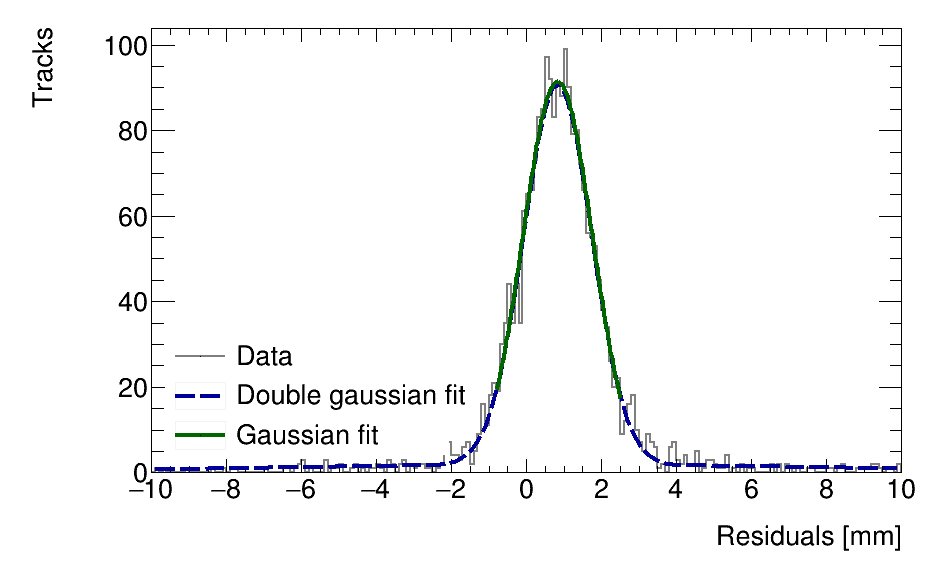
\includegraphics[width = \textwidth]{figures/figure_double_gaussian_quick_and_dirty_2900V_log_scale_gaussian_QL2C04_2900V_2021-02-08_2_xbin_10_ybin_5_100mm.png}
    \caption{Residual distribution for tracks on layer 1 built from hits on layers 3 and 4 for $x\in\left[-3.00, 97.00\right],  y\in\left[394.60, 494.60\right] mm$ fit with a double gaussian and a single gaussian in a range of $\pm$1 RMS from the histogram mean.}
    \label{fig:double_gaussian_example_fit}
\end{figure}

For all residual distributions in \SI{100}{\milli\meter} by \SI{100}{\milli\meter} bins on layer 1 built from hits on layers 3 and 4, the difference in gaussian and double gaussian means and standard deviations is shown in \ref{fig:double_gaussian_compare_fits}. Since the RMS of the residual means is lesser than \SI{50}{\micro\meter}, it is safe to use the Gaussian. Moreover, this is for the tracking combination with the worst extrapolation lever arm, and so the widest distribution of means; the interpolation combinations are narrower. It is expected that the gaussian standard deviation should be larger than the double gaussian standard deviation as shown because the gaussian distribution includes the effect of the noise tracks with large residuals, while the double gaussian models them separately. For this analysis, only the residual mean is of importance, so the systematic overestimate of the signal sigma by the gaussian fit can be allowed.

\begin{figure}
    \centering
    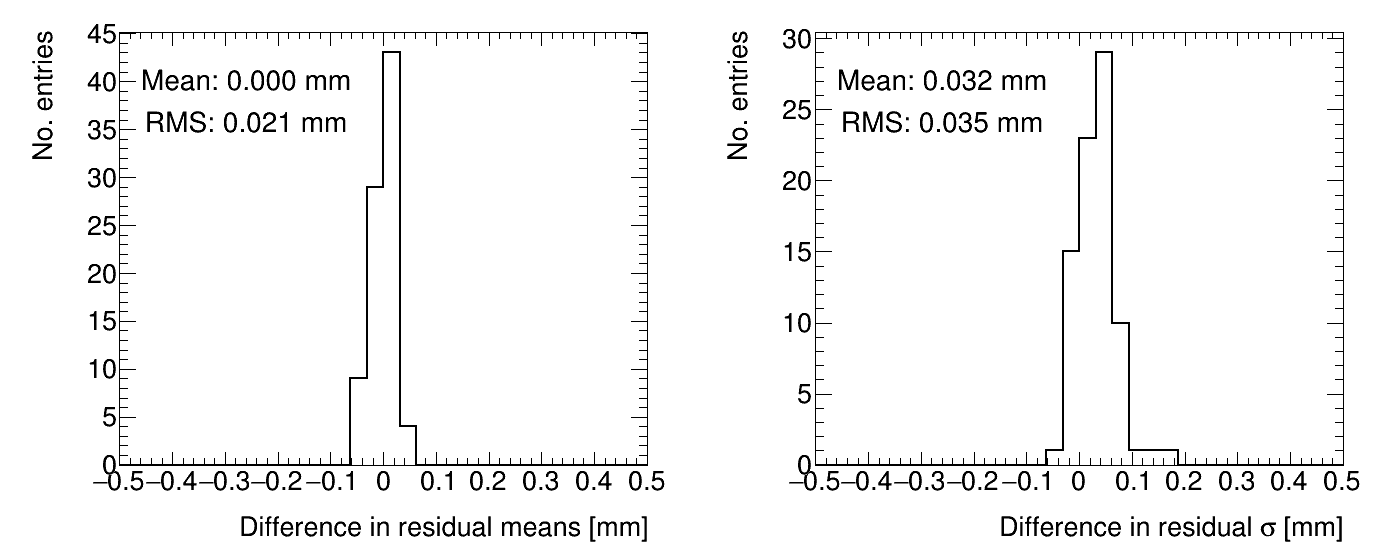
\includegraphics[width = \textwidth]{figures/figure_compare_residual_fits_QL2C04_2900V_2021-02-08_2_fit_range_mean_pm_RMS_minus_quick_and_dirty_2900V_log_scale_layer1_fixedlayers34.png}
    \caption{Difference in residual distribution means and standard deviations for a gaussian and double gaussian fit.}
    \label{fig:double_gaussian_compare_fits}
\end{figure}

